การวิจัยนี้มีเป้าหมายในการหาหัวข้อและทัศนคติของความคิดเห็นของผู้ใช้งานโปรแกรมที่อยู่ตาม app store โดยใช้วิธีการประมวลผลภาษาธรรมชาติ และการทำเหมืองข้อมูล
\begin{figure}[h]
	\centering
	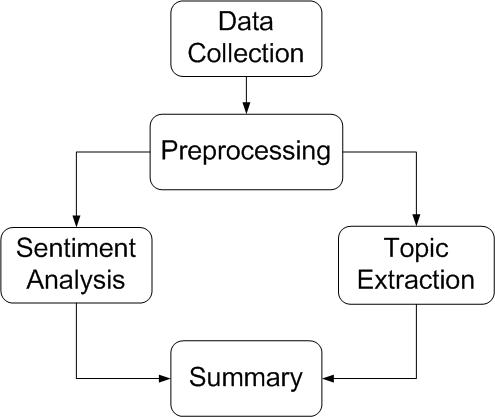
\includegraphics[width=.8\linewidth]{Process.jpg}
	\caption{Overview of approach}
	\label{fig:approachFig}
\end{figure}
Figure \ref{fig:approachFig} จะแสดงขั้นตอนทั้งหมดในการวิจัย โดยจะเริ่มตั้งแต่ 1. Data Collection 2. Prepossessing 3. Sentiment Analysis 4. Topic Extraction 5. Summary 
\subsection{Data Collection}

\begin{table}[h]
	\caption{no. of review in each app.}
	\label{table:NoOfReview}
	\centering
	\begin{tabular}{|c|r|}
		\hline
		Application & \multicolumn{1}{|c|}{no. of review} \\
		\hline
		Man Man & 1279\\
		\hline
		H-Tv & 691\\
		\hline
		K-mobile & 1055\\
		\hline
	\end{tabular}
\end{table}
เราได้รวบรวมข้อมูลความคิดเห็นของผู้ใช้งานจากโปรแกรมประเภทต่าง ๆ บน Google Play store โดยการรวบรวมจากบนหน้าเว็บไซต์สำหรับดาว์นโหลดโปรแกรมนั้น ๆ
โดยรวบรวมจากโปรแกรม "แม่น แม่น" (virtual keyboard), "H-Tv" (TV Online), "K-mobile" (Internet Mobile Banking) โดยเราได้รวบรวมข้อมูลในช่วง กุมภาพันธ์ 2015 - พฤษภาคม 2016 และ ช่วง มิถุนายน 2016 - สิงหาคม 2016 (นับจากวันที่ผู้ใช้งานแสดงความคิดเห็น) ซึ่งมีปริมาณข้อมูลตาม Table \ref{table:NoOfReview} โดยข้อมูลที่ผู้วิจัยได้รวบรวมมา ได้แก่ author, title, detail, rate, review-date ซึ่งแสดงตัวอย่างตาม Table \ref{table:review}

\begin{table*}[h]
	\caption{example of review}
	\label{table:review}
	\centering
	\begin{tabular}{|l|l|l|r|c|}
		\hline
		\multicolumn{1}{|c|}{author} &
		\multicolumn{1}{|c|}{title}&
		\multicolumn{1}{|c|}{review}&
		\multicolumn{1}{|c|}{rate}&
		\multicolumn{1}{|c|}{date}\\
		\hline
		โชคชัย มหาวงนันท์ & โชคชัย มหาวงศ์นันท์ & ใช้ได้ดีครับ & 5&10/04/2015\\
		\hline
		bie slow life &  & พักหลังนี่อัพบ่อยนะครับ & 4&09/19/2015\\
		\hline
		ornanohg Hongrrimon &  & ชอบค่ะใช้ง่าย มีตัวการ์ตูนให้ด้วย & 5&09/20/2015\\
		\hline
		Terdsak chompusri &  & เรียบง่ายแต่ใช้ได้ดีจริงๆครับชอบมาก & 5&09/22/2015\\
		\hline
		Worapote Panomauppatum & วรพจน์  พนมอุปถัมภ์ & ใช้ได้เยื่ยมมาก & 5&09/25/2015\\
		\hline
		Nate Makboon & เนตร มากบุญ & ดีมากครับ สะดวกดีแม่นสุดยอด & 5&09/24/2015\\
		\hline
	\end{tabular}
\end{table*}

%แต่สำหรับเจ้าของโปรแกรมนั้น ๆ สามารถนำข้อมูลเหล่านี้ออกมาได้จากหน้า console ของโปรแกรมนั้น ๆ ได้ทันที
\subsection{Prepossessing}
หลังจากที่เราได้ข้อมูลที่ต้องการแล้ว เราจะนำข้อมูลเหล่านั้นมาหา POS ก่อนเพื่อใช้ในการทำงานขั้นต่อไป แต่ก่อนที่เราจะหา POS ได้ เราจะต้องตัดประโยค และตัดคำก่อน
\subsubsection{sentence extraction}
เนื่องจากข้อมูลความคิดเห็น 1 ความคิดเห็นอาจจะไม่ได้มีเพียงประโยคเดียว ดังนั้นเราจึงจำเป็นต้องแบ่งประโยคออกมาเสียก่อน เนื่องจากประโยคภาษาไทยนั้นเราไม่มี pattern ที่ตายตัวในการแบ่งประโยคเหมือนอย่างภาษาอังกฤษ และในปัจจุบันมีคำสมัยใหม่เพิ่มขึ้นมาอีกมากมาย ทำให้ลำบากในการใช้เครื่องมือในการแบ่งประโยค อีกทั้งยังจำเป็นต้องใช้ corpus ที่มีข้อมูลของรูปประโยคที่ค่อนข้างมากเพื่อใช้ในการจำแนกประโยคต่าง ๆ ดังนั้นเราจึงใช้วิธี manual ในการแบ่งประโยค 

โดยเราใช้ pattern ในการแบ่งประโยคคือ\\ 
1. ถ้าเจอคำว่า "ครับ"/"ค่ะ" เราจะถือว่าเป็นการจบประโยค\\
2. ถ้าเจอคำว่า "แต่" เราจะถือว่าเป็นการขึ้นประโยคใหม่
\subsubsection{word segmentation}
เมื่อเราแบ่งประโยคเรียบร้อยแล้วเราจะนำประโยคที่ได้แต่ละประโยคมาตัดแยกคำเพื่อนำไปหา POS ต่อไป โดยในการตัดคำนั้นเราได้ใช้เครื่องมือที่ชื่อ LexTo ซึ่งพัฒนาโดย NECTEC เป็นซึ่งใช้วิธีการตัดคำแบบ longest matching 
ในการตัดคำ
\subsubsection{pos tagger}
เราหา pos ของคำโดยใช้ RDRPOStagger ซึ่งมี ORCHID เป็น corpus สำหรับการคำนวน
\subsection{Sentiment Analysis}
ส่วนนี้เป็นการนำประโยคที่มีการกำหนด pos ของคำแล้วมา คำนวนหาทัศนคติของประโยค โดยสำหรับการหา sentiment ของคำในภาษาไทยนั้นยังไม่มี corpus ที่เผยแพร่ ดังนั้นเราจึงเลือกใช้ SentiWordNet \cite{SentiWordNet} ซึ่งเป็น corpus สำหรับหา sentiment ของคำในภาษาอังกฤษ 

ดังนั้นขั้นตอนแรกของการหา sentiment ของงานวิจัยนี้จึงเป็นการแปลคำศัพท์จากไทย-อังกฤษ โดยเราเลือกใช้ LEXiTRON \cite{LEXiTRON} เป็นพจนานุกรมในการแปลคำศัพท์ โดยการหาคำที่มี POS ตรงกัน ทำให้เราได้ synonym ภาษาอังกฤษ

ขั้นต่อมาเราจะนำ synonym ที่ได้มาหา sentiment ใน SentiWordNet โดยค่าของ sentiment ที่ได้จะอยู่ในช่วง [-1,1] ดังตัวอย่างใน Table \ref{table:Top10sentiword}
แต่เนื่องจากค่าที่ได้จาก SentiWordNet เราพบว่า คำบางคำ ที่ให้ความรู้สึกในเชิงลบของรูปประโยค มีค่าที่ได้เป็นบวก ดังนั้นเราจึงจำเป็นต้องสร้างลิสต์คำที่คาดว่าให้ความรู้สึกเชิงลบ แล้วนำมาเทียบกับ sentiment ที่ได้ ถ้า sentiment ที่ได้เป็นบวก เราจะกลับค่า sentiment นั้นให้เป็นลบแทน และในกรณีที่มีคำว่า "ไม่" นำหน้าคำ ๆ นั้น เราก็จะกลับค่า sentiment ของคำนั้นแทน

จากนั้นเราจะหาค่า sentiment ของประโยคโดยการนำค่า sentiment ทั้งหมดของประโยคนั้น ๆ มาเฉลี่ยเป็นคะแนนของประโยค
\subsection{Topic Extraction}
ส่วนนี้เป็นส่วนที่อธิบายถึงวิธีการหาหัวข้อของประโยค โดยเราใช้วิธี LDA ในการค้นหาหัวข้อ ซึ่งจะทำหลังจากการหา pos ของคำ
โดยเรากำหนดให้ number of topic ที่ต้องการเป็น 20 เนื่องจากเราไม่ทราบหัวข้อที่แน่นอน จากนั้นเราจะเลือกหัวข้อที่เหมาะสมออกมาจากหัวข้อทั้งหมดที่ได้
%not finish
\subsection{Summary}
หลังจากที่เราได้กลุ่มคำของ topic ต่าง ๆ และ sentiment ของประโยคแล้ว เราจะรวมรวบประโยคที่มีคำตรงกับในกลุ่มคำของ topic เพื่อนำมาแสดงถึงคะแนน sentiment ของ topic นั้น ๆ และนำคะแนนที่ได้มาหาค่า absolute maximum เพื่อแสดงถึง sentiment รวมของหัวข้อนั้น ๆ ว่าคะแนนเป็นบวก หรือเป็นลบ Table\ref{table:topicManMan} แสดงถึงตัวอย่างคะแนนที่ได้จากการวิจัย

นอกจากนี้เรายังสามารถแจกแจงได้ว่าแต่ละหัวข้อมี ประโยคที่มีทัศนคติเป็นบวก หรือเป็นลบ อยู่อย่างละกี่ประโยคได้อีกด้วย


\begin{table}[h]
	\renewcommand{\arraystretch}{1.3}
	\caption{Top 10 sentiment of each word in Man Man app}
	\label{table:Top10sentiword}
	\centering
	\begin{tabular}{|c|c|c|c|}
		\hline
		\multicolumn{2}{|c|}{negative} &
		\multicolumn{2}{|c|}{positive}\\
		\hline
		{\selectlanguage{thai}ลบ} & -0.33621 & {\selectlanguage{thai}น่ารัก} & 0.21843\\
		\hline
		{\selectlanguage{thai}เสียดาย} & -0.17095 & {\selectlanguage{thai}รัก} & 0.20107\\
		\hline
		{\selectlanguage{thai}เกลียด} & -0.16666 & {\selectlanguage{thai}เพลิน} & 0.17563\\
		\hline
		{\selectlanguage{thai}ดุ} & -0.15297 & {\selectlanguage{thai}ดี} & 0.16622\\
		\hline
		{\selectlanguage{thai}สายตายาว} & -0.12500 & {\selectlanguage{thai}สวย} & 0.16310\\
		\hline
		{\selectlanguage{thai}ขยายตัว} & -0.09566 & {\selectlanguage{thai}สุดยอด} & 0.15476\\
		\hline
		{\selectlanguage{thai}ห่วย} & -0.09071 & {\selectlanguage{thai}มันส์} & 0.15085\\
		\hline
		{\selectlanguage{thai}ปวด} & -0.07943 & {\selectlanguage{thai}ไว} & 0.12500\\
		\hline
		{\selectlanguage{thai}เสียใจ} & -0.07943 & {\selectlanguage{thai}ชอบ} & 0.12246\\
		\hline
		{\selectlanguage{thai}ไม่ดี} & -0.06995 & {\selectlanguage{thai}สนุก} & 0.10604\\
		\hline
	\end{tabular}
\end{table}
